\section{Fundamentação Teórica}
\subsection{Modelos de cores}

\begin{frame}{Introdução}
\begin{itemize}
    \item A cor tem a característica poderosa de funcionar como um descritor
    \item Os seres humanos têm a capacidade de discernir milhares de tonalidades e intensidades
    \item A percepção humana das cores se dá pela ativação de células nervosas que enviam mensagens ao cérebro sobre brilho (\textit{brightness}), matiz (\textit{hue}) e saturação (\textit{saturation})
    \item As cores podem ser especificadas por modelos matemáticos em tuplas de números em um sistema de coordenadas
    \item Dois tipos: os modelos aditivos e subtrativos
\end{itemize}
\end{frame}

%------------------------------------------------------
\begin{frame}{Modelo de Munsell}
\begin{figure}[!h]
  \centering
  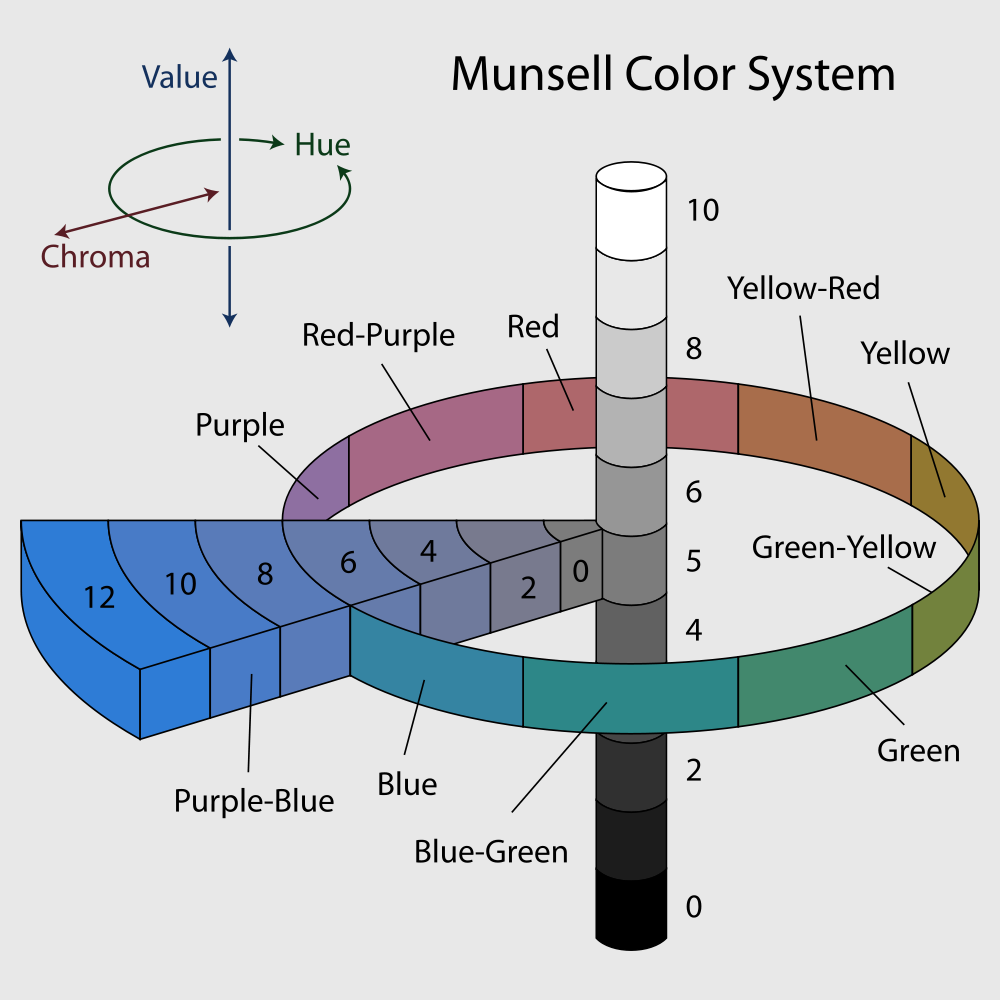
\includegraphics[width=.55\textwidth]{munsell-system}
\end{figure}
\end{frame}

%------------------------------------------------------
\begin{frame}{Diagrama de cromaticidade CIE 1931}
\begin{columns}
\column{0.5\textwidth}
\begin{itemize}
    \item Primeiro modelo matemático de especificação numérica da cor
    \item Componente de luminância Y; X e Z de cromaticidade (tristímulus)
    \item Derivações do CIE XYZ: \textbf{CIE 1976 $L^*u^*v^*$} e \textbf{1976 CIE $L^*a^*b^*$}
\end{itemize}
\column{0.5\textwidth}
\begin{figure}[!h]
  \centering
  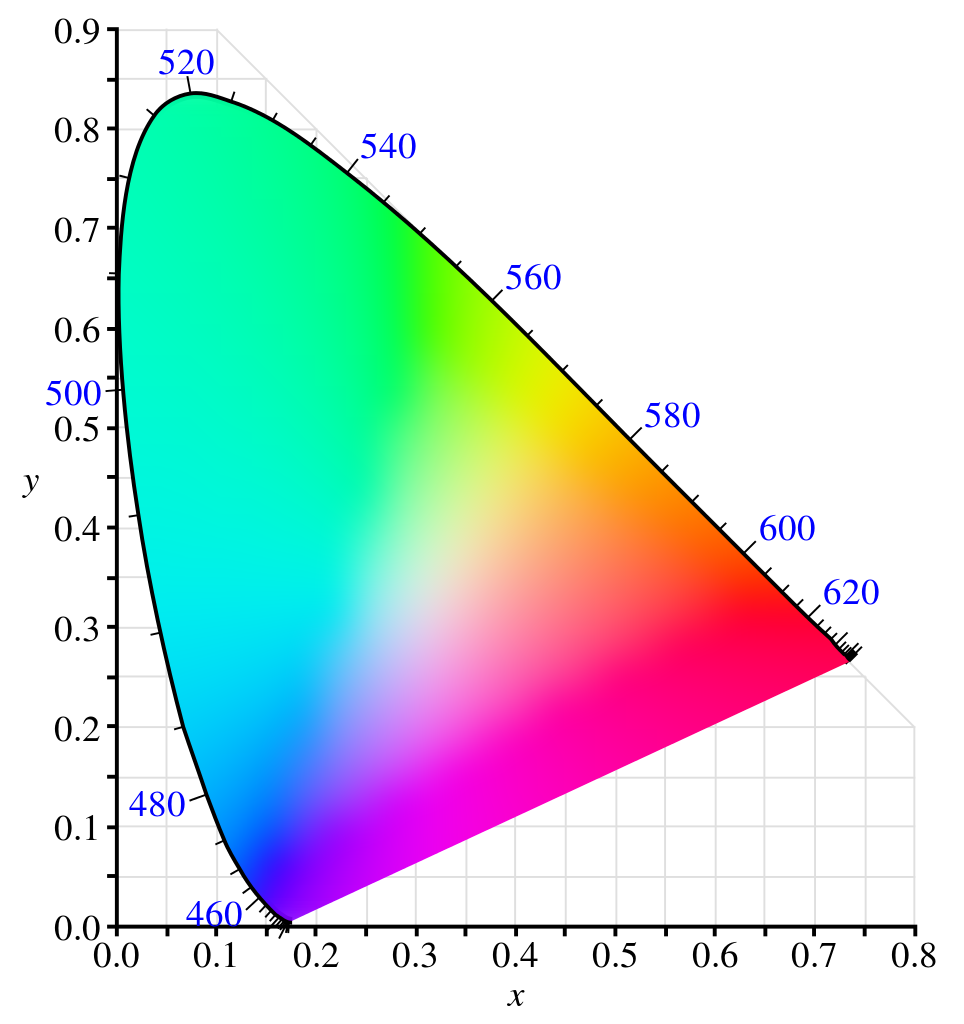
\includegraphics[width=1\textwidth]{cie-cromaticity-diagram}
\end{figure}
\end{columns}
\end{frame}

%------------------------------------------------------
\begin{frame}{Modelo RGB}
\begin{columns}
\column{0.5\textwidth}
\begin{itemize}
    \item Modelo de cores aditivo
    \item Baseado na teoria tricromática de Thomas Young e Hermann Helmholtz em meados do século 19
\end{itemize}
\column{0.5\textwidth}
\begin{figure}[!h]
  \centering
  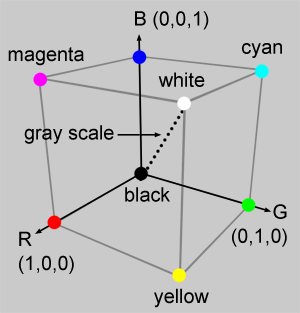
\includegraphics[width=.9\textwidth]{rgb-cube}
\end{figure}
\end{columns}
\end{frame}

%------------------------------------------------------
\begin{frame}{Modelos da família YUV}
\begin{itemize}
    \item Y = luminância, U = Azul - Y, V = Vermelho - Y
    \item Utilizado em sistemas de transmissão analógica de televisão nos padrões PAL e SECAM
    \item YCbCr é um modelo desta família e é largamente utilizado em vídeos digitais.
\end{itemize}
\begin{equation*}
  \begin{bmatrix}
    Y \\ Cb \\ Cr
  \end{bmatrix} = 
  \begin{bmatrix}
     0.299 &  0.587 &  0.114 \\
    -0.169 & -0.331 &  0.5   \\
     0.5   & -0.419 & -0.081 \\
  \end{bmatrix}
  \begin{bmatrix}
    R \\ G \\ B
  \end{bmatrix}
\end{equation*}
\end{frame}

%------------------------------------------------------
\begin{frame}{Modelos da família HSI}
\begin{itemize}
    \item  (I)ntensidade é decomposta da informação de crominância
\end{itemize}
\begin{align}
\begin{split}
  H &=  \begin{cases}
            60\ffrac{(G - B)}{M - m}, & \text{se}\ M = R\\[0.7em]
            60\ffrac{(B - R)}{M - m} + 120, & \text{se}\ M = G\\[0.7em]
            60\ffrac{(R - G)}{M - m} + 240, & \text{se}\ M = B
       \end{cases}
  \\[0.5em]
  S &=  \begin{cases}
            \ffrac{(M - m)}{M}, \quad &\text{se}\ M \neq 0\\[0.7em]
            0, \quad &\text{caso contrário}\\
       \end{cases}
  \\[0.5em]
  V &= M
\end{split}
\end{align}
\end{frame}

%------------------------------------------------------
\subsection{Teoria fuzzy}
\begin{frame}{Introdução}
\end{frame}

%------------------------------------------------------
\begin{frame}{Conjuntos \emph{fuzzy}}
\end{frame}

%------------------------------------------------------
\begin{frame}{Números \emph{fuzzy}}
\end{frame}

%------------------------------------------------------
\begin{frame}{Funções de pertinência}
\end{frame}

%------------------------------------------------------
\begin{frame}{Funções de pertinência}
\end{frame}

%------------------------------------------------------
\subsection{Classificadores}
\begin{frame}{Máquinas de Vetores Suporte (SVM)}
\end{frame}

%------------------------------------------------------
\begin{frame}{$k$-Vizinhos Mais Próximos ($k$-NN)}
\end{frame}

%------------------------------------------------------
\begin{frame}{Árvores de decisão}
\end{frame}